%!TEX root = informe.tex

\IEEEPARstart{F}{i}nalizada la enumeraci\'on de los problemas que motivan la investigaci\'on sobre el tema y la adici\'on de una breve explicaci\'on del problema a trabajar y de la justificación teórica detrás del método de interpolación, nos dedicaremos a desarrollar con mayor precisi\'on cada m\'etodo n\'umerico en cuesti\'on. Recordemos que estos métodos intentan atacar el problema de construir, a partir de un video filmado en tiempo real, nuevos frames que den la sensaci\'on de que el video original ha sido ralentizado (efecto de \emph{slowmotion}), o, aún mejor, filmado con una cámara de alta frecuencia.

\subsection{Aclaraciones \'utiles para la comprensi\'on del desarrollo}

Antes de comenzar con la explicaci\'on de los m\'etodos queremos definir ciertas frases o palabras claves que ocupar\'an terreno en el resto de la secci\'on:

\begin{itemize}
	\item \textit{Frame original}: Cuadro que pertenece al video original, es decir, aquel que no contiene los frames agregados que conciben al efecto de c\'amara lenta.
	\item \textit{Frame artificial}: Cuadro que se realizar\'a a partir del procedimiento que cada m\'etodo vaya planeando. Siempre tiene a cierta distancia, tanto a derecha como izquierda, frames originales.
	\item \textit{Cantidad de frames a adjuntar}: Entero que indica cu\'antos cuadros artificiales le adicionaremos entre cada par de frames originales. Lo denotaremos con las letras $fr$.
	\item \textit{Matriz frame}: Aunque no se hablar\'a de este nombre en particular, es fundamental aclarar que en cualquier comentario acerca de los valores o p\'ixeles de un frame, se lo est\'a modelando como una matriz de $m \times n$ (resoluci\'on del video) que lleva los valores del $0$ al $255$ inclusive (escala de grises).
    \item \textit{P\'ixel}: Transladamos esta palabra asociada a la imagen digital al campo del \'algebra lineal. Por lo tanto, se lo considerar\'a como un componente de la matriz frame cuyos valores estan restringido en el rango $[0;255]$.
\end{itemize}

Para la explicación de todos los métodos consideramos dado (como parámetros del problema) el video sobre el cual trabajar (con su resolución $m \times n$) y la cantidad $fr$ de frames a generar entre cada par de frames del original.

Además, dado $t \in \mathbb{R}$ definiremos lo siguiente para ayudarnos en las definiciones más formales:

\begin{align*}
    &original(t) \text{ sii } t \text{ coincide con el instante de tiempo de un frame original}\\
    original(t) \Rightarrow\ &frame(t)=\text{el frame original del instante $t$}\\
    \neg original(t) \Rightarrow\ &anterior(t) = \max_{k}(original(k) \wedge k < t)\\
    \neg original(t) \Rightarrow\ &siguiente(t) = \min_{k}(original(k) \wedge k > t)\\
    \neg original(t) \Rightarrow\ &resto(t) = t-anterior(t)\\
    0 \leq i < m \wedge 0 \leq j < n \Rightarrow&\ f[i,j] =\text{el valor de brillo de píxel en la posición $(i, j)$ para un frame $f$}
\end{align*}


\subsection{Los m\'etodos propuestos}
\subsubsection{Cuadro m\'as cercano}

Este m\'etodo se basa en una idea simplista, muy sencilla de implementar, y que nos permitirá tener una base para establecer comparaciones con métodos más ``inteligentes''. A pesar de esto, puede resultar precisa para ciertos tipos de videos, como por ejemplo, la filmaci\'on de un objeto inmóvil.

\subsubsection*{\bf{Intuición}}

Como lo indica el subt\'itulo de la secci\'on, la idea del método es que cada frame artificial es una copia de su frame original más cercano en términos temporales. Para cada frame a generar el método calcula cuál es dicho ``vecino más cercano'' y luego copia la im\'agen de dicho frame al frame artificial a generar. 

De esta manera, habr\'a al menos $fr/2$ copias de cada frame original. En caso que se decida agregar una cantidad impar, se opta por fragmentar en dos partes de $fr/2$ y $fr/2+1$ cuadros. En la figura \ref{fig:vecino} vemos un ejemplo conciso de lo explicado. La cantidad de cuadros a agregar es de $fr = 22$, por lo que se lo divide en dos particiones de $11$ frames artificiales cuya imagen corresponder\'a al frame original m\'as cercano (el marr\'on o blanco).

\begin{figure}[h!]
  \centering
    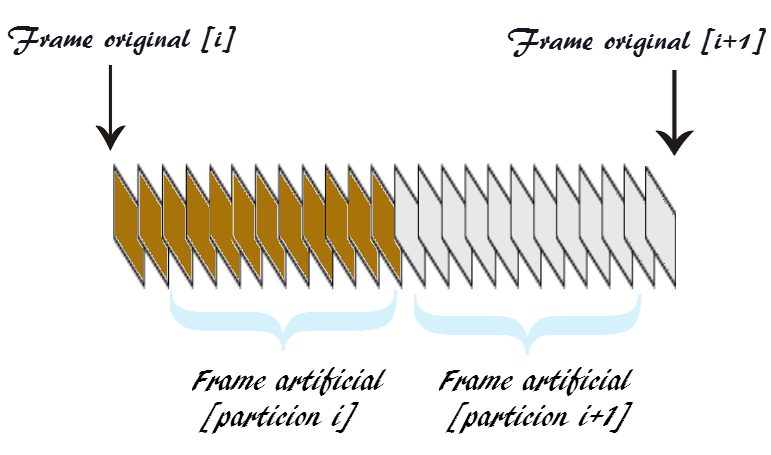
\includegraphics[width=0.55\textwidth]{VecinoCercano.png}
     \caption{Ejemplo de vecino m\'as cercano}\label{fig:vecino}
\end{figure}
\noindent

Volviendo al an\'alisis del video en su totalidad, se repite el anterior procedimiento para cada par de frames en el orden establecido por la secuencia del video. De tal forma se obtienen los frames artificiales, consiguiendo una nueva filmaci\'on con el efecto de \textit{slowmotion} que queríamos. 

\subsubsection*{\bf{Perspectiva matem\'atica}}

\textbf{¿Qu\'e relaci\'on tiene este m\'etodo con el concepto de interpolar?} A pesar de ser muy sencillo, este método está usando cierta forma de interpolación. Si consideramos cada píxel $(i, j)$ del video a lo largo del tiempo, obtenemos para cada uno una lista de pares $f_{i,j}(t)=y$ donde $t$ es el instante de un frame original y $y$ el valor de brillo del píxel $(i,j)$ de dicho frame. El método propuesto interpola dichos puntos usando 

\[
f_{i,j}(t) = 
\left\{
    \begin{array}{ll}
        frame(t)_{i,j} & \mbox{si } original(t) \\
        frame(anterior(t))_{i,j} & \mbox{si } resto(t) \leq fr/2 \\     
        frame(siguiente(t))_{i,j} & \mbox{si } resto(t) > fr/2
    \end{array}
\right.
\]

Es fácil ver que la función interpola efectivamente los puntos $f_{i,j}(t)=y$, aunque lo hace de modo ``pobre'': para cada par de frames originales tiene una discontinuidad entre ellos a distancia $fr/2$, que será percibida como un ``salto'' en las imágenes del video. El único caso en que esto no ocurre es cuando los frames considerados son idénticos, por lo que arriesgamos que es el caso en que el método mejor se comportará.

\subsubsection{Interpolaci\'on lineal}

Compartiendo con \emph{vecino m\'as cercano} la idea de trabajar píxel a píxel con cada par de frames para eventualmente obtener el video deseado con su respectivo efecto, este método puede propocionar ciertas mejoras a la hora de trabajar con videos con movimiento\footnote{Que, entendemos, es el caso de la mayoría de los videos, exceptuando quizás los subidos a YouTube para compartir música.}.

\subsubsection*{\bf{Intuición}}
El m\'etodo se centra en tomar crear un interpolador lineal segmentado por cada píxel del video, cuyos puntos interpolados son los valores de brillo del píxel en los frames originales. Por ende, tendremos por cada par de frames originales $m \times n$ polinomios de grado uno, que usaremos para conocer los valores intermedios entre los dos cuadros originales y gererar así los píxeles de los frames artificiales.

En la figura \ref{fig:lineal} se puede observar el efecto producido por una interpolación de este estilo.

\begin{figure}[h!]
  \centering
    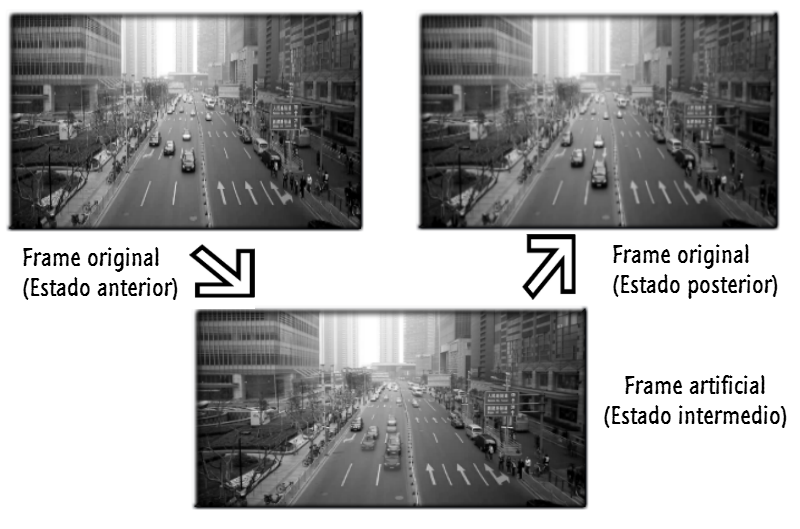
\includegraphics[width=0.65\textwidth]{InterpolacionLineal.png}
     \caption{Muestra de interpolaci\'on lineal con un solo frame intermedio}\label{fig:lineal}
\end{figure}
\noindent

\subsubsection*{\bf{Perspectiva matem\'atica}}
Nuevamente consideramos para cada píxel una lista de pares $f(t)=y$. Aplicando lo visto en la Introducción teórica, para cada píxel construimos $S_0, \ldots, S_{n - 1}$ polinomios de grado a lo sumo 1 (con $n$ cantidad total de frames del video) tal que $S_p$ interpola $t_p=y_p$ y $t_{p + 1}=y_{p+1}$ para cada $t_p$ instante de un frame original. Luego, definimos la siguiente funci\'on:
 
\[
f(t) = 
\left\{
    \begin{array}{ll}
        S_0(t)  & \mbox{si } t \in [t_{0}, t_1] \\
        \hspace{0.3cm}\vdots \\     
        S_{n - 1}(t) & \mbox{si } t \in [t_{n - 1}, t_n]
    \end{array}
\right.
\]

Como ya dijimos, habrá una de estas $f_{i,j}$ por cada píxel $(i,j)$, pero nos restringimos a definirla para un único para evitar la notación $_{i,j}$ en todas las ecuaciones.

Cada $S_p$ se define como la siguiente recta:

$$S_p(t) = y_p + (y_{p+1} - y_p) * \frac{t - t_0}{t_1 - t_0}$$

Donde $y_{p} = frame_p[i,j]$, $y_{p+1} = frame_{p+1}[i,j]$, $t_0=anterior(t)$ y $t_1=siguiente(t)$. Es importante aclarar que siempre se debe evaluar esta funci\'on dentro del rango $(t_0, t_1)$, es decir, los puntos intermedios.

Para una mayor comprensi\'on, representaremos gr\'aficamente el método. Supongamos que tenemos el algoritmo que instancia una funci\'on $S_{p}$, tomando la información de un par de p\'ixeles de igual posici\'on (por ejemplo $(1,2)$) en $frame_0$ y $frame_1$, y la evalúa en $fr$ puntos para generar píxeles artificiales. Asumiendo $fr = 2$, observamos en la figura \ref{fig:intSimple} el resultado.

Si lo usamos considerando ahora múltiples frames ($frame_0 \ldots frame_6$) generamos 6 splines $S_0, \ldots, S_5$ y 12 frames artificiales como se puede ver en la figura \ref{fig:intConjunta}.

\begin{figure}[h!]
  \centering
    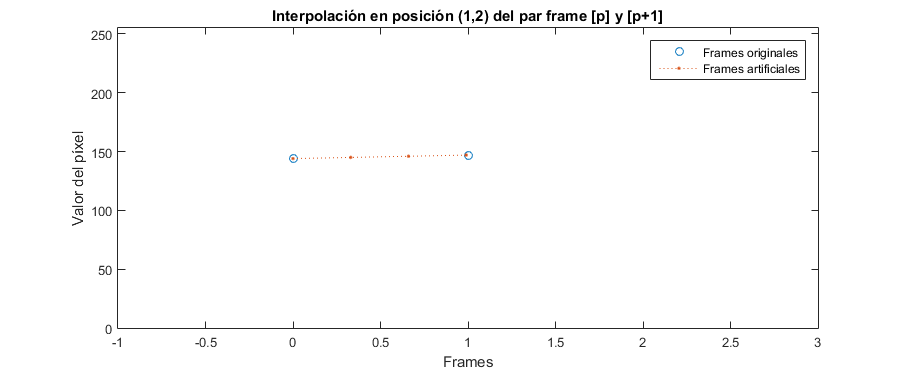
\includegraphics[width=0.85\textwidth]{InterpolacionSimple.png}
     \caption{Resultado de interpolar usando 2 frames}\label{fig:intSimple}
\end{figure}
\noindent

\begin{figure}[h!]
  \centering
    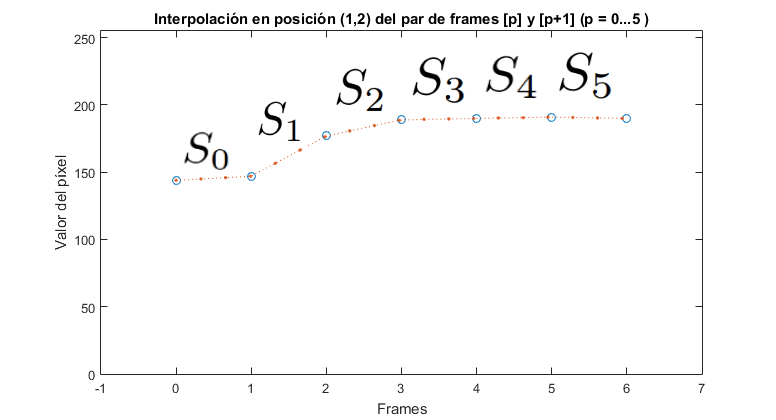
\includegraphics[width=0.75\textwidth]{InterpolacionConjunta.png}
     \caption{Resultado de interpolar usando 7 frames}\label{fig:intConjunta}
\end{figure}
\noindent

\subsubsection{Construcción mediante interpolación por splines (c\'ubica)}

Continuando con la idea de conseguir los frames artificiales o intermedios mediante la creación y evaluación de polinomios para cada píxel, pasamos a utilizar polinomios de grado 3. Por lo dicho en la introducción teórica creeríamos que esto puede brindar resultados m\'as satisfactorios en la construcci\'on del video final, aunque habr\'a que confirmar esto durante la experimentaci\'on.

\subsubsection*{\bf{Intuición}}

Siendo \'este el tercer y \'ultimo m\'etodo a desarrollar, podemos abstraernos de ciertos detalles que fueron previamente explicados.

Ya hemos dicho que pertenece a la familia de los interpoladores por segmentos. En principio, se podr\'ia pensar que el método no cambia su metodolog\'ia con respecto al anterior. Nos limitaremos aquí a expresar en qué se diferencian.

A diferencia del m\'etodo de Interpolaci\'on lineal, este método varía sus resultados dependiendo de todos los frames considerados para hacer el spline, es decir, no genera cada $S_k$ únicamente en función del valor del píxel en los frames $k$ y $k+1$, sino que todos los frames influyen en los coeficientes de la funci\'on $S_k$, y su evaluación en el punto $t$ puede variar dependiendo de qué frames fueron considerados. Esto se debe, intuitivamente, a que el método utiliza la información de todos los frames para generar cada función $S_{i,j}$, combinándola en un único sistema de ecuaciones\footnote{ver sección \ref{sec:splines}}.

Una opción sencilla en su implementación es usar todos los frames del video para generar el spline. El problema es que el sistema matricial a resolver puede ser muy grande, potencialmente excediendo las capacidades de memoria de las computadoras comunes y trayendo inconvenientes no deseados al uso del método. Queda entonces la aplicación de una alternativa: crear múltiples splines de a bloques. Es decir, tomar cierta cantidad de frames y definirla como el \textit{tamaño de bloque}, para luego generar un spline por cada bloque.

\subsubsection*{\bf{Perspectiva matem\'atica}}
Considerando como un nuevo tamaño el tamaño de bloque (que eventualmente podría ser igual a la cantidad de frames del video, dando lugar a un único spline por píxel) generamos un spline por píxel por bloque. Los puntos a interpolar serán el tiempo $t$ y el valor del brillo $y$ de dicho píxel en todos los frames del bloque.

Usando la equivalencia vista en la Introducción teórica (del problema de encontrar los coeficientes de un spline con el de resolver un sistema de ecuaciones lineal) podemos generar la matriz asociada al sistema para cada spline a generar y resolver el sistema usando eliminación gaussiana normalmente. Eso nos da como resultado los coeficientes $(a_i,b_i,c_i,d_i)$ de cada polinomio cúbico $S_k$ de los que componen el spline. Luego basta hacer
$$
S(t) = 
\left\{
    \begin{array}{ll}
        S_0(t)  & \mbox{si } t \in [t_{0}, t_1] \\
        \hspace{0.3cm}\vdots \\     
        S_{n - 1}(t) & \mbox{si } t \in [t_{n - 1}, t_n]
    \end{array}
\right.
$$

para generar cada spline $S$.

